\documentclass[letterpaper,twocolumn,10pt]{article}
\usepackage{usenix2019_v3}

% to be able to draw some self-contained figs
\usepackage{tikz}
\usepackage{amsmath}
\usepackage{graphicx}

% inlined bib file
\usepackage{filecontents}

\graphicspath{ {./images/} }

%-------------------------------------------------------------------------------
\begin{filecontents}{\jobname.bib}
%-------------------------------------------------------------------------------


  
@InProceedings{vcg,
author = {Nick Dunn and John Murray},
booktitle = {VCG [VisualCodeGrepper] - Source code security scanning tool.},
title = VCG [VisualCodeGrepper] - Source code security scanning tool.,
year = {2019},
publisher = {https://github.com/nccgroup/VCG},
journal = {GitHub repository},
howpublished = {\url{https://github.com/charlespwd/project-title}},
commit = {4f57d6a0e4c030202a07a60bc1bb1ed1544bf679}
}
\end{filecontents}

%-------------------------------------------------------------------------------
\begin{document}
%-------------------------------------------------------------------------------

%don't want date printed
\date{}

% make title bold and 14 pt font (Latex default is non-bold, 16 pt)
\title{\Large \bf Density Based Clustering for Hierarchical and Autonomous Fog Architecture}

%for single author (just remove % characters)
\author{
{\rm Robin C.\ Ward}\\
PhD Student\\
Auburn University\\
Auburn, Alabama 36849\\
Email: rcw0024@auburn.edu\\
} % end author

\maketitle

%-------------------------------------------------------------------------------
\begin{abstract}
%-------------------------------------------------------------------------------
As the complexities of computer security continue to grow every year, the need for a streamlined and fast way to perform code review continues to increase. Luckily, there are a lot of tools available to help expedite the review process, one of which is called  Visual Code Grepper%
\footnote{\url{https://github.com/nccgroup/VCG}} (VCG). VCG is an open-source Windows tool that was written in visual Basic .NET. VCG is an automated static code security review tool that can handle scans of many languages, such as: C/C++, Java, VB, and PL/SQL. VCG really excels in environments where code is being pushed out quickly and the need for review of common issues is critical. There are other tools%
\footnote{\url{https://security.web.cern.ch/recommendations/en/code_tools.shtml}} that can also help in situations like this, but VCG is a very fast and easy to install application. However, after careful review of VCG, it was determined that there are a few areas where improvements could be made. Those areas are the backup of local configuration files, restore of local configuration files, and most importantly, the download of updated security definitions and bad functions to search for. The following text is an explanation of the configuration files that was extracted from the readme.md~\cite{vcg} file.

\begin{verbatim}
put psuedocode here
\end{verbatim}

\end{abstract}


%-------------------------------------------------------------------------------
\section{Introduction}
%-------------------------------------------------------------------------------

In the following sections, many areas will be covered such as the new features added to the VCG tool, the importance of them, some of the code%
\footnote{VCG uses Visual Basic .NET} that was required to implement them as well as future improvements. In addition to explaining the new additions that were added to the VCG tool, each following section will include a subsection that will also contain possible improvements and/or advancements that could be added on top of what has already been done. These additions, though may seem small, should prove to be a worthy addition to the VCG tool. It is also recommended that the reader download%
\footnote{\url{https://sourceforge.net/projects/visualcodegrepp}} and install the VCG tool and become familiar with all of its features. A list of other similar tools as well as the VCG tool can be found See Figure~\ref{fig:backup} for the location of the new button.

\subsection{Possible Improvements}
\begin{description}
\item[configuration file select] One possible improvement that would make the backup feature better would be the addition of a multi-select backup. This would allow the user to select which configuration files they would like to backup. 
\item[progress bar] Another improvement which may prove to be useful would be the addition of a progress bar when backing up the local files. Even though the process is very fast, sometimes a visual indicator is still nice to have, especially if the files grow in size as time goes on.

\end{description}

%-------------------------------------------------------------------------------
\section{Backup}
%-------------------------------------------------------------------------------

The first feature that was added is the backup functionality. This should prove to be a very valuable addition to the VCG tool as it will allow users to safely, securely, and quickly backup any of the configuration files that are locally hosted. to accomplish this, a new button was added to the main VCG form application. The main idea behind this is that the VCG tool would look at the configuration file directory, then proceed to upload all of the configuration files to an FTP server. For simplicity purposes, the remote file location was utilizing FTP, but any method of file transfer could have been implemented, and in a production environment, this would be highly recommended. 

\begin{figure}[h]
\centering
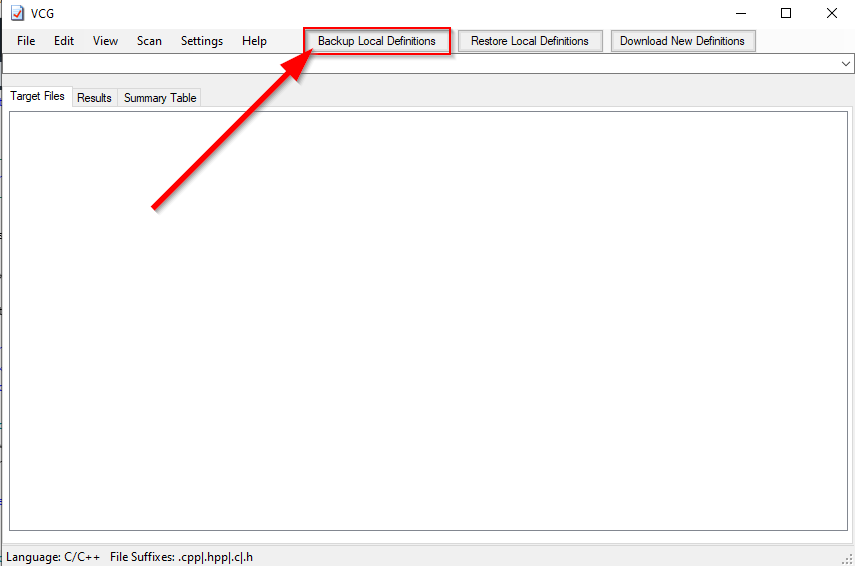
\includegraphics[width=0.45\textwidth]{backup}
\caption{\label{fig:backup}Location of the new "Backup Definitions" button.}
\end{figure}

The Visual Basic (VB) code was straight forward for the most part. After adding an action to the button, the following code was needed to be added to the frmMain.vb in order to execute the upload%
\footnote{In order to keep the logic concise for this paper, only the C++ code was included. However, the same logic would apply for every language.}. 



%-------------------------------------------------------------------------------
\section{Restore}
%-------------------------------------------------------------------------------

\begin{figure}[h]
\centering
\includegraphics[width=0.45\textwidth]{restore}
\caption{\label{fig:restore}Location of the new "Restore Definitions" button.}
\end{figure}

\subsection{Possible Improvements}
\begin{description}
\item[configuration file select] One possible improvement that would make the restore feature better would be the addition of a multi-select restore. This would allow the user to select which configuration files they would like to restore.
\item[configuration file save path] Another possible improvement that would make the restore feature better would be the addition of a multi-select restore. This would allow the user to select which configuration files they would like to restore.

\item[progress bar] Another improvement which may prove to be useful would be the addition of a progress bar when restoring the files from the server to the local machine. Even though the process is very fast, sometimes a visual indicator is still nice to have, especially if the files grow in size as time goes on.

\end{description}

%-------------------------------------------------------------------------------
\section{Download New Definitions}
%-------------------------------------------------------------------------------

The last and most important feature added was the ability to download new configuration files that contain new definitions and bad functions that were released by the developer. This is a very important addition to the VCG tool because it will now allow users to get updated threats to search for in seconds. 

\begin{figure}[h]
\centering
\includegraphics[width=0.45\textwidth]{download}
\caption{\label{fig:download}Location of the new "Download New Definitions" button.}
\end{figure}



\bibliographystyle{plain}
\bibliography{\jobname}

%%%%%%%%%%%%%%%%%%%%%%%%%%%%%%%%%%%%%%%%%%%%%%%%%%%%%%%%%%%%%%%%%%%%%%%%%%%%%%%%
\end{document}
%%%%%%%%%%%%%%%%%%%%%%%%%%%%%%%%%%%%%%%%%%%%%%%%%%%%%%%%%%%%%%%%%%%%%%%%%%%%%%%%

%%  LocalWords:  endnotes includegraphics fread ptr nobj noindent
%%  LocalWords:  pdflatex acks